%---------- Quarto Capítulo ----------
\chapter{Protocolo de Autenticação e Autorização proposto}\label{cap:Protocolo}
\section{Introdução}
%A Polícia Civil do Distrito Federal, diante da necessidade de compartilhar suas informações com órgão parceiros, no intuito de possibilitar que os sistemas possam ser integrados de forma eficiente e principalmente segura busca estabelecer uma arquitetura de referência para a adoção de uma arquitetura orientada a serviços. Essa arquitetura deve primar pela segurança, haja vista a criticidade e sensibilidade das informações que são tratadas no âmbito da PCDF.

%Dessa forma, optou-se por adotar a tecnologia de Web Services usando o protocolo REST para implementar SOA na instituição. Neste caso, estudos específicos foram realizados com vistas a estabelecer uma política de segurança eficiente que possibilite o fornecimento dos serviços e promova a integração com os órgãos parceiros.
A Polícia Civil do Distrito Federal, diante da necessidade de compartilhar suas informações com órgão parceiros, no intuito de possibilitar que os sistemas possam ser integrados de forma eficiente e principalmente segura busca estabelecer uma arquitetura de referência para a adoção de uma arquitetura orientada a serviços. Essa arquitetura deve primar pela segurança, haja vista a criticidade e sensibilidade das informações que são tratadas no âmbito da PCDF.

Dessa forma, optou-se por adotar a Web services \emph{RESTFul} para implementar SOA na Instituição. Neste caso, estudos específicos foram realizados com vistas a estabelecer uma política de segurança eficiente que possibilite o fornecimento dos serviços e promova a integração com os órgãos parceiros. Sendo assim, surgiu a necessidade da criação de um protocolo seguro e personalizado de autenticação e autorização que atenda às necessidades da PCDF.

\section{Requisitos do Protocolo}\label{sec:reqprotocolo}

O protocolo de autenticação e autorização proposto deverá ser aderente a arquitetura REST, de forma que possa permitir que os serviços ofertados pela Divisão de Tecnologia possam ser acessados por um número relativamente grande de clientes. Os requisitos inerentes ao protocolo são descritos nesta seção.

\begin{enumerate}[RQ1]

\item Para promover a segurança de sessão, toda comunicação entre o cliente e o servidor será realizada utilizando HTTPS \emph{(Hypertext Transfer Protocol over Secure Sockets Layer)}, usando o SSL/TLS para garantir a confidencialidade e integridade para a sessão. Para isso será usado o certificado digital X.509, emitido por uma autoridade de certificação, para encriptar as comunicações e garantir a autenticidade do servidor e do cliente. Devendo os clientes realizar a validação do certificado antes de interagir com o servidor.

\item Será utilizado a criptografia assimétrica para promover a segurança na troca de mensagens realizada entre o Cliente e a PCDF. Todas as mensagens deverão ser assinadas digitalmente. Para isso, será utilizado uma função hash, com o algoritmo SHA(Secure Hash Algorithm).

\item O protocolo deverá permitir acesso aos serviços apenas ao pessoal autorizado, de forma que a autenticação e autorização, siga padrões definidos na política de segurança. Sendo que para ser autenticado e autorizado o usuário deverá apresentar credenciais válidas. Essas credenciais deverão ser criptografadas, assinadas e enviadas no cabeçalho do protocolo HTTPS. Devendo ser escalável em termos de sobrecarga, tamanho do domínio de proteção e de manutenção. Além disso, ele deverá permitir a preservação de privacidade, uma vez que para proteger os clientes e fornecedores de recursos de entidades maliciosas, suas interações deverão revelar o mínimo de informações possíveis.

\item A autenticação e autorização será baseada em desafios e resposta, que serão elaborados a partir da apresentação de declarações de identidade (Claims). Tal requisito torna mais flexível o gerenciamento da identidade do usuário, uma vez que possibilita ao administrador desabilitar credenciais que tenham sido comprometidas de forma transparente ao usuário.

\item A política de autenticação e autorização proposta no protocolo será estabelecida por meio de contrato onde serão definidos todas as regras que deverão ser atendidas pelos usuário e pelo fornecedor do serviço.

    Dessa forma, para que qualquer usuário possa ter acesso aos serviços ofertados pela Divisão de Tecnologia da PCDF ele deverá concordar com um contrato prévio de acesso. Devendo primeiramente ser cadastrado e ter definido quais são seus privilégios de acesso/autorização. Uma vez cadastrado o usuário deverá informar os dados que possam comprovar sua identidade no momento da autenticação de forma que ele possa ser autorizado de acordo com o seus privilégios.

    No momento do credenciamento será gerado para o cliente múltiplas credenciais, que serão utilizadas no processo de autenticação e autorização, essas informações serão compartilhados entre o Cliente o Servidor de Autenticação e Autorização e o Servidor REST. Além disso, o Contrato poderá ter acesso a múltiplos serviços. A Figura ~\ref{fig:diagrama_relacionamento} apresenta o relacionamento entre o contrato, credenciais e serviços.

\begin{figure}[!htb]
    \centering
    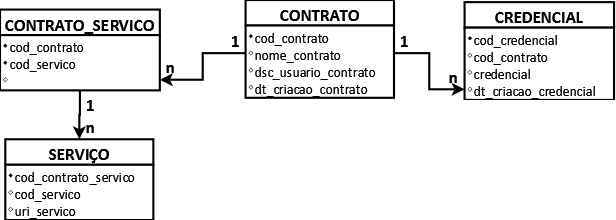
\includegraphics[width=0.8\textwidth]{modelo_relacionamento_contrato1.png}
    \caption{Diagrama de relacionamento entre contrato, credenciais e usuários}
    \label{fig:diagrama_relacionamento}
\end{figure}

\end{enumerate}


%Para a implementação de segurança em aplicações REST, verificou-se que ela passa basicamente pela aplicação de segurança em protocolos \emph{HTTP}, que oferece dois tipos de autenticação:  \emph{Basic} e \emph{Digest}.

%A autenticação Basic é um modelo baseado no desafio e resposta, sendo utilizada por servidores HTTP para validar a autenticação~\cite{franks1999}. Desta forma, quando o cliente tenta acessar algum recurso protegido, a sua identidade é requerida pelo servidor, o cliente então fornece a resposta codificada em base64 no header \emph{HTTP},  se a resposta for correta ela terá acesso ao sistema. Porém, por não criptografar o desafio, estando esse apenas codificado, faz com que ele seja vulnerável e sujeito a ataques, como por exemplo, os de repetição.

%Já na Digest, o processo é o mesmo que na autenticação básica. Sendo que seu mecanismo de autenticação é um pouco mais complexo, uma vez que ele gera um HASH, geralmente utilizando o algoritmo MD5, do desafio que será enviado pelo servidor ao cliente ~\cite{franks1999}. Apesar de ser mais seguro do que a autenticação básica, autenticação HTTP Digest também é vulnerável à ataques, como por exemplo o man-in-the-middle.  Para evitar esse problema, deve ser empregado a segurança na camada de transporte~\cite{Webber10}.

\section{Arquitetura do Protoloco}\label{sec:ArqProtocolo}

A arquitetura do protocolo proposto é apresentada na Figura~\ref{fig:arquiteturaprotocolo}. O protocolo é composto por quatro componentes: Cliente, Servidor de Autenticação e Autorização, Servidor REST, e Banco de Dados de Autenticação e Autorização.

\begin{figure}[!htb]
    \centering
    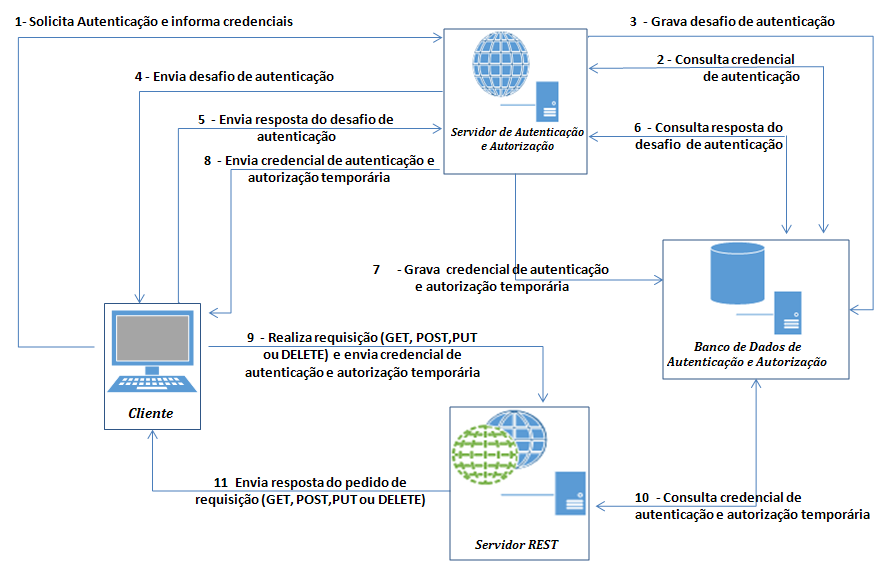
\includegraphics[width=0.8\textwidth]{arquitetura_protocolo.png}
    \caption{Fluxo do protocolo de autenticação/autorização proposto, 1º cenário.}
    \label{fig:arquiteturaprotocolo}
\end{figure}

Os componentes da arquitetura são detalhados a seguir.

Cliente: O componente Cliente na arquitetura do protocolo representa as Instituições ou Órgãos conveniados, que após firmar um contrato, podem consumir os serviços ofertados pela PCDF.

Servidor de Autenticação e Autorização: Este componente tem um papel fundamental na arquitetura do protocolo, pois é nele que o gerenciamento de autenticação e autorização é realizado. Desta forma, o servidor de Autenticação e Autorização é responsável por realizar os processos de verificação e validação de credenciais, criação dos desafios de autenticação, criação de \emph{tokens} JSON e a criação e o gerenciamento das credenciais de autenticação e autorização temporárias, que são utilizados pelos clientes para consumir os serviços requisitados.

Servidor REST: Esse é um servidor de fachada que abstrai toda lógica necessária para o consumo dos serviços.Neste servidor estão concentrados os serviços REST disponibilizados pela PCDF. Desta forma, quando um Cliente necessita acessar um serviço, primeiramente ele deve ser autenticado e autorizado no servidor de Autenticação e Autorização. Após esse processo, o Cliente faz a requisição ao servidor de REST, que realiza as verificações necessárias para saber se o Cliente tem privilégios ou não para acessar o serviço. Ele acessa a base de dados de Autenticação e Autorização para confirmar as credenciais de autenticação e autorização temporária informadas e caso elas sejam válidas ele permite que o Cliente acesse o serviço requerido. Um ponto importante a ser destacado é que os desenvolvedores, ao desenvolver um serviço, não necessitam ter preocupações de segurança, uma vez que é esse componente que realiza esse atividade.

Banco de Autenticação e Autorização: Servidor de banco de dados que contém a estrutura de banco de dados necessário  para o funcionamento dos serviços de autenticação e autorização. É neste servidor que são gravados as credenciais, usuários, os desafios e as credenciais de autorização e autenticação temporária.


\subsection{Visão geral do protocolo de Autenticação e Autorização proposto}

Para ter acesso a API \emph{REST}, referente aos serviços ofertados, o cliente deverá ser autenticado e autorizado a acessar o serviço. Para isso, será usado a autenticação baseada em \emph{tokens} de segurança, que são recipientes de reivindicações da autoridade emissora. Os \emph{tokens} de segurança utilizados serão os \emph{Web Tokens} no formato \emph{JSON}. Esse, ao contrário dos tokens \emph{SAML}, que são baseados em \emph{XML}, são mais compactos e, portanto mais adequados para serem usados em um cabeçalho \emph{HTTP}. Além disso, todas as mensagens deverão ser assinadas e criptografadas de forma assimétrica. O processo de autenticação e autorização é descrito em dois cenários distintos. No primeiro cenário, representado na figura ~\ref{fig:protocoloseguro}, o Cliente, não está autenticado. No segundo cenário, ele está autenticado e possui uma credencial de autorização. %Esse último é representado na figura ~\ref{fig:cenario2}.

\subsubsection{Primeiro cenário}
No primeiro cenário, o cliente não está autenticado, e irá solicitar a autenticação pela primeira vez, conforme descrito a seguir:
\newline
\begin{figure}[!htb]
    \centering
    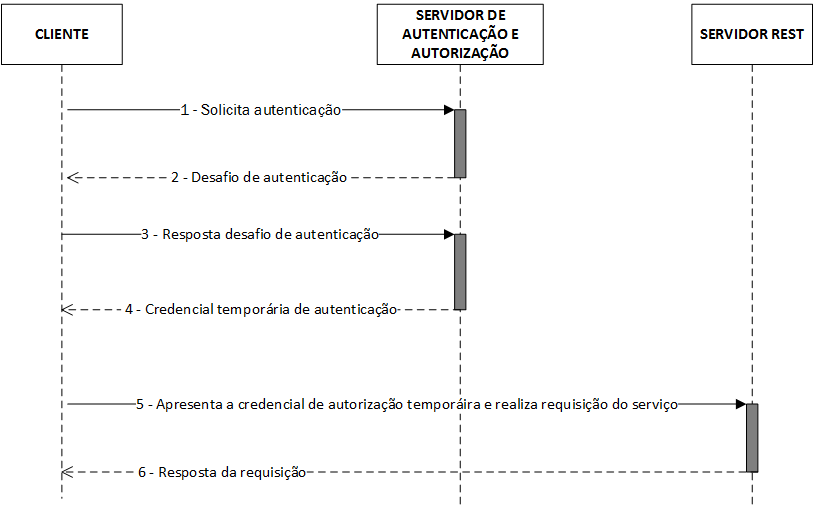
\includegraphics[width=1.0\textwidth]{fluxo_autenticacao.png}
    \caption{Fluxo do protocolo de autenticação/autorização proposto, 1º cenário.}
    \label{fig:protocoloseguro}
\end{figure}


O protocolo tem início quando o Cliente envia uma solicitação de autenticação ao servidor de Autenticação e Autorização. Esse pedido é realizado por meio de uma mensagem (mensagem 1 da Figura~\ref{fig:protocoloseguro}) que contém um \emph{token} JSON, enviado no cabeçalho HTTP da requisição REST. O \emph{token} contém uma credencial, extraída de forma aleatória da tabela de credenciais do Cliente. O token é assinado digitalmente pelo Cliente e cifrado com a chave pública do servidor de Autenticação e Autorização. É importante frisar que tanto o Cliente quanto o servidor de Autenticação e Autorização possuem as mesmas tabelas de credenciais e de serviços, pois elas são geradas no momento de assinatura do contrato de prestação do serviço.

Na segunda mensagem, ao receber uma solicitação de autenticação, o servidor de Autenticação e Autorização extrai o token cifrado com sua chave privada e verifica a autenticidade e integridade da requisição por meio da verificação da assinatura digital do Cliente.  Se houver qualquer problema, uma mensagem de erro HTTP (código 401): usuário não autorizado, é retornada ao Cliente.
Outra verificação que é realizada é a do \emph{timestamp}, que se refere ao tempo de envio da mensagem, se ela tiver sido enviada em um período de tempo superior ao pré-estabelecido no contrato, o Cliente também recebe uma mensagem de erro HTTP de usuário não autenticado.

Caso não haja problemas, procede-se com o processo de validação da credencial informada, que consiste em consultar a credencial em uma base de dados e se a credencial for válida e estiver associada ao Cliente, o Servidor de Autenticação e Autorização gera um desafio de autenticação. Tal desafio consiste em fazer uma busca aleatória à tabela de credenciais e selecionar um código de credencial que esteja associado ao Cliente. Em seguida grava-se o desafio, a data e hora de geração do desafio e a resposta que o Cliente deverá fornecer. um \emph{token} JSON, contendo o código do desafio, o código da credencial e um \emph{timestamp} representando a data e hora de criação do desafio, é enviado ao Cliente, assinado digitalmente pelo servidor de Autenticação e Autorização e cifrado com a chave pública do Cliente que está solicitando a autenticação.

Na terceira mensagem, após receber o desafio do servidor de Autenticação e Autorização, o Cliente, extrai o token cifrado com sua chave privada e verifica a autenticidade e integridade da requisição por meio da verificação da assinatura digital do servidor de Autenticação e Autorização. Em seguida verifica o \emph{timestamp}, cujo objetivo é o de verificar se a mensagem foi enviada em um período de tempo superior ao pré-estabelecido no contrato. Se houver qualquer problema, o processo de autenticação atual é descartado e inicia-se um novo processo de autenticação.

Caso não haja problemas, o Cliente verifica e responde o desafio solicitado, enviando-o, juntamente com um \emph{timestamp} e o código do serviço, que ele deseja consumir, para o Servidor de Autenticação e Autorização por meio de um \emph{token} JSON, que é assinado digitalmente pelo Cliente e cifrado com a chave pública do servidor de Autenticação e Autorização.

Na quarta mensagem, o servidor de Autenticação e Autorização recebe a resposta do desafio de autenticação, decifra o token e verifica a autenticidade e integridade da requisição por meio da verificação da assinatura digital do Cliente.  Não ocorrendo problemas, inicia-se o processo de verificação da resposta. A primeira verificação que é realizada refere-se ao tempo de geração do desafio, por meio do \emph{timestamp}. Se a resposta tiver sido enviada em um período de tempo superior ao pré-estabelecido em contrato, o servidor de Autenticação e Autorização envia uma mensagem de erro HTTP (código 401): usuário não autorizado, ao Cliente. Caso contrário, ele procede com a verificação do desafio que consiste em realizar uma consulta na tabela de desafios verificando se a resposta dada é a mesma que a esperada. Caso a resposta esteja correta o servidor de Autenticação e Autorização autentica o Cliente. Em seguida ele verifica, pelo código do serviço requisitado se o Cliente tem privilégios necessários para consumir o serviço requisitado.

Se a resposta for positiva, o servidor de Autenticação e Autorização gera uma credencial de autenticação e autorização temporária para o serviço solicitado. Ela é gravada em uma tabela de credencias de autorização temporária juntamente com a data e hora de criação, data de expiração e o código do cliente. A tabela de credencias de autorização temporária será acessada pelo Servidor REST  para verificar quais privilégios a entidade requisitante do serviço tem acesso e se ela está autenticada. O token, contendo a credencial de autenticação e autorização temporária, é  assinado digitalmente pelo servidor de Autenticação e Autorização   e cifrado  com a chave pública do Cliente. Após esse processo ele é enviado ao Cliente.

Caso a resposta do desafio esteja em desacordo com a esperada ou se o Cliente não tiver privilégios suficientes para acessar o serviço requisitado, ele recebe uma mensagem de erro HTTP (código 401): usuário não autorizado.
É importante frisar que a credencial de autenticação e autorização temporária será gerada apenas para o serviço que o Cliente tenha solicitado e possua o privilégio de acesso para utilizá-la. Ela será válida por um período  de tempo que será definido no momento da assinatura do contrato de prestação de serviço, entre o órgão conveniado e a PCDF.

Na quinta mensagem, o Cliente, extrai o token cifrado com sua chave privada e verifica a autenticidade e integridade da requisição por meio da verificação da assinatura digital do servidor de Autenticação e Autorização. Em seguida verifica o \emph{timestamp}, cujo objetivo é o de verificar se a mensagem foi enviada em um período de tempo superior ao pré-estabelecido no contrato. Se houver qualquer problema, o processo de autenticação atual é descartado e inicia-se um novo processo de autenticação.

Caso não haja problemas, o Cliente verifica a data e hora de validade da credencial de autorização temporária para saber se ela é válida. Confirmada sua validade, ele envia ao servidor REST, a requisição do serviço que deseja consumir juntamente com a credencial de autenticação e autorização temporária. O token de autenticação e autorização temporária é assinado com a chave privada do Cliente e cifrado com chave pública do servidor REST, sendo enviado no cabeçalho da requisição.

Finalmente, após receber a requisição, o Servidor REST, extrai o token cifrado com sua chave privada e verifica a autenticidade e integridade da requisição por meio da verificação da assinatura digital do servidor de Autenticação e Autorização. Em seguida verifica o \emph{timestamp}, para saber se a mensagem foi enviada em um período de tempo superior ao pré-estabelecido no contrato. Não havendo problemas, o Servidor REST verifica se a credencial de autenticação e autorização temporária é valida. Para isso, ele realiza uma consulta na tabela de credenciais temporárias, com a finalidade de confirmar se a credencial informada não expirou, se  foi realmente gerada para o Cliente e se ela está associada ao serviço solicitado.

Caso não haja problemas, o Cliente recebe os dados referentes à sua requisição. Havendo qualquer problema ele recebe uma mensagem de erro HTTP (código 401) de usuário não autorizado.

%Já no segundo cenário, que é representado na figura ~\ref{fig:cenario2}. O Cliente, já possui uma credencial de autorização temporária, neste caso ele deverá apresentá-la sempre que desejar consumir algum serviço que ele tenha acesso.
\subsubsection{Segundo cenário}

Já no segundo cenário, o Cliente, já possui uma credencial de autorização temporária, neste caso ele deverá apresentá-la sempre que desejar consumir algum serviço que ele tenha acesso conforme descrito a seguir:

Neste caso, o Cliente envia um token contendo uma credencial temporária no cabeçalho da requisição do serviço que deseja consumir, ao Servidor de REST.

O servidor de REST, recebe o token de autenticação e autorização, faz a verificação na tabela de credenciais temporárias para saber se o Cliente possui uma credencial válida, em caso positivo ele verifica quais são os privilégios de autorização da credencial, se ele tiver permissão para acessar o serviço, sua requisição é atendida.

Caso a credencial não seja válida ou tenha expirado o Cliente é redirecionado para o servidor de Autenticação e Autorização para que possa se autenticar novamente e obter uma nova credencial conforme descrito no primeiro cenário. %Esse processo é descrito no fluxo alternativo da figura ~\ref{fig:cenario2}.

%\begin{figure}[!htb]
%    \centering
%     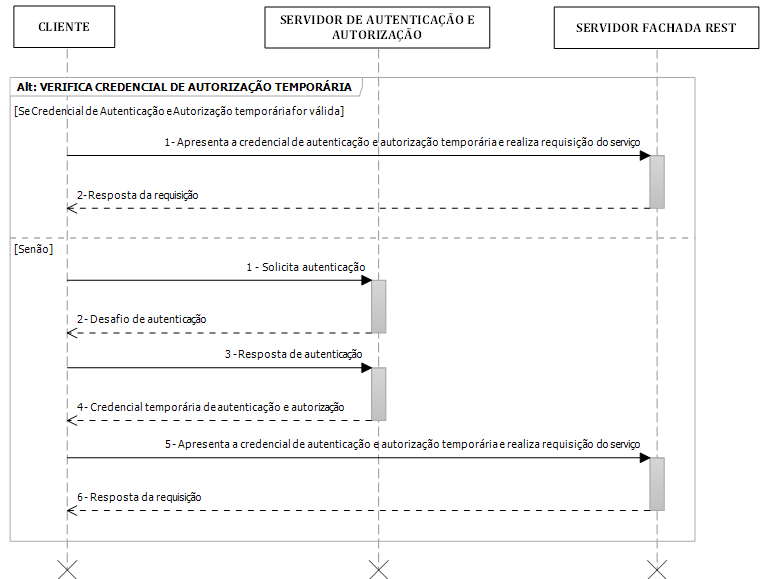
\includegraphics[width=0.8\textwidth]{cenario2_autenticacao.png}
%     \caption{Fluxo do protocolo de autenticação/autorização proposto, 2º cenário.}
%     \label{fig:cenario2}
%\end{figure}


\section{Formalização do protocolo}

O emprego de avaliações mais formais na área de criptografia não é recente. Grande parte dos trabalhos nesta área foram desenvolvidos na década de 90~\cite{Meadows95}. O emprego destes métodos possibilita uma análise completa do protocolo criptográfico e sua função principal é especificar se os objetivos propostos pelos autores são alcançados.

Neste trabalho, o protocolo proposto foi descrito formalmente, utilizando a lógica BAN, com o intuito de favorecer a comunicação e o entendimento utilizando uma linguagem mais precisa. Além disso, a propriedade de terminação com a geração da credencial temporária de autenticação e autorização foi verificada com um programa escrito em Prolog (ver Apêndice em anexo).


\section{Lógica BAN}

A lógica BAN foi desenvolvida por Burrows, Abadi e Needham em 1989, ela e uma das mais populares para a análise de crenças e de conhecimento entre os participantes dos protocolos criptográficos. É a primeira lógica a analisar formalmente os protocolos criptográficos,principalmente os de autenticação e distribuição de chaves~\cite{Burrows1990}.

\subsection{Notação básica}
Na lógica BAN, existem vários tipos distintos de objetos tais como entidades ou partes que se comunicam, chaves de criptografia e fórmulas lógicas. Uma fórmula lógica é uma versão idealizada da mensagem original, e às vezes ela pode ser referenciada como uma declaração lógica. Normalmente, os símbolos A, B e S denotam entidades ou participantes; $Kab$, $Kas$ e $Kbs$ denotam chaves compartilhadas; Ka, Kb e Ks denotam chaves públicas e $Ka^{-1}$, $Kb^{-1}$ e $Ks^{-1}$ denotam as chaves privadas dos participantes. Já $Na$, $Nb$ e $Ns$ são os identificadores gerados pelos participantes. As construções mais frequentemente utilizadas são apresentadas na Tabela~\ref{tab:notacaobasicaBAN}:

 \newcommand{\RHQuery}{\textbf{[???]}}
\newcommand{\RHRemark}[1]{\textbf{[#1]}}
\newcommand{\Believess}[2]{{#1}\mathrel{\textbf{\mid\equiv}}{#2}}
\newcommand{\Seess}[2]{{#1}\mathrel{\textbf{\triangleleft}}{#2}}
\newcommand{\Saids}[2]{{#1}\mathrel{\textbf{\mid\sim}}{#2}}

\newcommand{\Believes}[2]{{#1}\mathrel{\textbf{acredita}}{#2}}
\newcommand{\Sees}[2]{{#1}\mathrel{\textbf{recebeu}}{#2}}
\newcommand{\Said}[2]{{#1}\mathrel{\textbf{disse}}{#2}}
\newcommand{\Controls}[2]{{#1}\mathrel{\textbf{controla}}{#2}}
\newcommand{\Fresh}[1]{{#1}\,\textbf{novo}}
\newcommand{\Share}[3]{{#1}\stackrel{#2}{\longleftrightarrow}{#3}}
\newcommand{\ShareSecret}[3]{{#1}\stackrel{#2}{\rightleftharpoons}{#3}}
\newcommand{\PubKey}[2]{{}\stackrel{#1}{\mapsto}{#2}}
\newcommand{\Secret}[3]{{#1}\stackrel{#2}{\leftrightharpoons}{#3}}
\newcommand{\Encrypt}[2]{\{\,{#1}\,\}_{#2}}
\newcommand{\EncryptFrom}[3]{\{\,{#1}\,\}_{#2}^{#3}}
\newcommand{\Attach}[2]{\langle {#1}\rangle_{#2}}

%  \begin{tabular}{cp{16cm}}
\begin{table}[h]
    \begin{tabular}{|l|p{10cm}|}
    \hline
    \textbf{\emph{Expressão }}         & \textbf{\emph{Leitura/Significado}}                                                                               \\ \hline
    ${P}\mid\equiv{X}$               & $\Believes{P}{X}$: $P$ crê em $X$, ou $P$ acredita que $X$ é verdadeiro \\ \hline
    ${P}\triangleleft{X}$            & $\Sees{P}{X}$:Alguém enviou uma mensagem para $P$ contendo $X$ ou de outra forma $P$ recebeu $X$   \\ \hline
    ${P}\mid\sim{X}$                 & $\Said{P}{X}$:$P$ disse uma vez $X$. A entidade $P$ em algum momento enviou uma mensagem incluíndo a declaração $X$.\\ \hline
    ${P}\Rightarrow {X}$                 & $\Controls{P}{X}$:$P$ tem jurisdição sobre $X$. Onde $P$ é uma autoridade sobre $X$ é deve ser confiável \\ \hline
    \#(X)                            & novo$(X)$: a fórmula novo $X$, ela não foi usada numa mensagem anterior à execução protocolo atual.  \\ \hline
    $\Share{P}{k}{Q}$                & (lê-se ``k é uma chave satisfatória para $P$ e $Q$''). A chave $k$ nunca será descoberta por qualquer participante, exceto por P, Q ou por alguém em quem eles confiam \\ \hline
    $\{{X}\}_K$                  & fórmula $X$ foi cifrada com a chave $K$. As mensagens cifradas somente são legíveis e verificáveis pelo possuidor da chave \\ \hline
    $\ShareSecret{P}{k}{Q}$         & ${k}$ é o segredo compartilhado entre ${P}$ e ${Q}$ e possivelmente também com as entidades de confiança deles. Somente ${P}$ e ${Q}$ podem usar k para provar suas identidades \\ \hline
    $\PubKey{K}{P}$:               & ${k}$ é a chave pública de ${P}$  \\ \hline
    \end{tabular}
    \caption {Notação básica Lógica BAN, adaptação de ~\cite{Burrows1990}.}
\label{tab:notacaobasicaBAN}
\end{table}



\subsection{Postulados lógicos}

No estudo de protocolos de segurança é importante diferenciar o tempo das demonstrações ou eventos.  Haja vista que se isso não for observado, problemas, como a não detecção  do  reenvio de mensagens,  poderá acontecer.  Segundo~\cite{Burrows1990}, a lógica BAN trata dessa distinção dividindo-a em duas épocas: presente, que é o tempo durante a execução do protocolo, e o passado,  que refere-se às mensagens enviadas antes da execução do protocolo, o que faz com que elas sejam rejeitadas, uma vez que não são confiáveis .  Essa divisão de tempo é suficiente para facilitar o entendimento de como a lógica pode ser manipulada.
Para realizar a análise dos protocolos de segurança a lógica BAN possui uma serie de postulados lógicos, regras~\cite{Burrows1990}. Alguns deles  são descritos  a seguir:

\begin{enumerate}[ A )]

 \item Regra de significado da mensagem. Esta regra faz parte da interpretação das mensagens
    A1.1. Para as chaves secretas compartilhadas:
    \begin{displaymath}
        \infer
        {{P}\mid\equiv{{Q}\mid\sim{X}}}
        {{P}\mid\equiv{\Share{P}{k}{Q,}}& {P}\triangleleft{\Encrypt{X}{k}}}
        %{\Believes{P}{\Said{Q}{X}}}
        %{\Believes{P}{\Share{P}{k}{Q,}}&\Sees{P}{\Encrypt{X}{k}}}
    \end{displaymath}

    Se $P$ acredita que $k$ é uma chave satisfatória para se comunicar com $Q$ e se $P$ recebeu a mensagem $X$ cifrada com a chave $k$, então $P$ acredita que $Q$ uma vez disse $X$

    A1.2. De forma similar, aplicada a para as chaves públicas:

    \begin{displaymath}
        \infer
        {{P}\mid\equiv{{Q}\mid\sim{X}}}
        {{P}\mid\equiv{\PubKey{K}{Q}}& {P}\triangleleft{\Encrypt{X}{k ^{-1}}}}
                %{\Believes{P}{\Said{Q}{X}}}
                %{\Believes{P}{\Share{P}{k}{Q,}}&\Sees{P}{\Encrypt{X}{k}}}
    \end{displaymath}



\item Regra de verificação do identificador. Essa regra verifica se a mensagem é recente, se foi enviada durante a execução atual do protocolo e consequentemente, se o emissor acredita nela.

  \begin{displaymath}
    \infer
    {{P}\mid\equiv{{Q}\mid\equiv{X}}}
    {{P}\mid\equiv{\#(X),}& {P}\mid\equiv{{Q}\mid\sim{X}}}
    %{\Believes{P}{\Believes{Q}{X}}}
    %{\Believes{P} novo$(X),$ &\Believes{P}{\Said{Q}{X}}}
  \end{displaymath}

   Se $P$ acredita que $X$ é novo e $P$ acredita que em algum momento $Q$ disse $X$,então $P$ também acredita que $Q$ acredita em X.

\item Regra da jurisdição. Esta regra representa a confiança e a autoridade de uma entidade sobre as declarações.
\begin{displaymath}
    \infer
    {{P}\mid\equiv{X}}
    {{P}\mid\equiv{{Q}\Rightarrow {X},}& {P}\mid\equiv{{Q}\mid\equiv{X}}}
   % {\Believes{P}{X}}
   % {\Believes{P}{\Controls{Q}{X},} &\Believes{P}{\Believes{Q}{X}}}
  \end{displaymath}

   Se $P$  acredita que $Q$ tem jurisdição sobre a declaração $X$ e $P$ acredita que $Q$ acredita em $X$, então $P$ confia na declaração $X$.

\end{enumerate}

Estes são alguns dos principais postulados utilizados na construção da análise formal de protocolos criptográficos. A utilização destas regras juntamente com as notações descritas na sessão anterior possibilita que a crença dos participantes de um protocolo possa ser declarada.

\section{Análise formal do protocolo proposto}
Nesta sessão será realizado a análise formal do protocolo de autenticação e autorização proposto, utilizando a lógica BAN.

Na lógica BAN a análise de um protocolo é dividida em quatro etapas: A idealização do protocolo, que é originada a partir do protocolo original. As hipóteses, que são a suposições a respeito do estado inicial, nessa etapa são definidas as fórmulas lógicas que estão ligadas às declarações do protocolo, as declarações que são afirmações sobre o estado do sistema. As regras de inferência ou postulados lógicos que são aplicadas para os pressupostos e as afirmações a fim de descobrir as crenças detidas pelas partes no protocolo. %Normalmente, as premissas incluem as declarações sobre bens essenciais e partilha, geração de uso único e de confiança entre os diretores. nalanisisisisii %%http:www.tml.tkk.fi/Opinnot/Tik-110.501/1995/ban.html

\subsection{Idealização do protocolo}
\newcommand{\HT}[3]{\{\,{#1}\,\}\,{#2}\,\{\,{#3}\,\}}
\newcommand{\Msg}[3]{{#1}\longrightarrow{#2}:\,{#3}}

Para especificar o protocolo formalmente foram utilizadas algumas notações para representar os elementos participantes. Logo, os símbolos ${A}$, ${B}$ e ${C}$ são utilizadas para representar respectivamente as entidades, elementos participantes, que trocam mensagens: Cliente, Servidor REST e Servidor de Autenticação e Autorização. As chaves públicas das entidades ${A}$, ${B}$ e ${C}$ são representadas respectivamente por ${Ka}$, ${Kb}$ e  ${Kc}$. Já as chaves privadas, seguindo o mesmo pressuposto, são representadas pelos símbolos ${{Ka} ^{-1}}$, ${{Kb} ^{-1}}$ e ${{Kc} ^{-1}}$. Os elementos ${Cred_A}$ e ${Cod_{Srv_A}}$ representam respectivamente a credencial utilizada pela entidade ${A}$ e o código que identifica o serviço que a entidade ${A}$ está requerendo.

O desafio gerado pela entidade ${C}$ é enviado a entidade ${A}$ e representado pela fórmula ${N_{CA}}$ que corresponde aos elementos: Código do Desafio gerado pela entidade ${C}$ e Código da Credencial aleatória da entidade ${A}$. A resposta do desafio gerada pela entidade ${C}$ à entidade ${A}$ é representado  pelo símbolo ${Resp_{AC}}$ que corresponde aos elementos: Código do Desafio gerado pela entidade ${C}$ e Credencial Solicitada da entidade ${A}$. ${Ts_A}$ e ${Ts_C}$ são respectivamente os \emph{timestamps} emitidos pelas entidades ${A}$ e ${C}$.

O símbolo ${Msg_{AC}}$ representa o resumo da mensagem enviada pela entidade ${A}$ a entidade ${C}$,  ${Msg_{CA}}$ representa o resumo da mensagem enviada pela entidade ${C}$ a entidade ${A}$ e ${Msg_{AB}}$ representa o resumo da mensagem enviada pela entidade ${A}$ a entidade ${B}$. O elemento ${H}$ representa o \emph{hashing} aplicado a uma mensagem utilizando o algoritmo SHA3.

E finalmente, o símbolo ${Exp_A}$ representa a data/hora  de expiração da Credencial Temporária de autorização e autenticação, ${C_{Aut}}$ corresponde à credencial temporária de autorização e autenticação gerada para a entidade A e ${Req_A}$, que refere-se à requisição de serviço de A ( Get, Put, Post ou Delete).

Para especificar formalmente um protocolo de segurança utilizando a lógica BAN, é necessário primeiro idealizar o protocolo, objeto da análise, e a partir da aplicação dos postulados e das suposições iniciais verificar se ele atinge ou não o seu objetivo. A idealização do protocolo proposto e descrito na figura ~\ref{fig:protocoidealizado} e representa o fluxo de troca de mensagens executado pelo protocolo. Todas as mensagens são consideradas na análise, pois utilizam criptografia assimétrica desde a primeira troca de mensagens.

\begin{figure}[!htb]
    \centering
    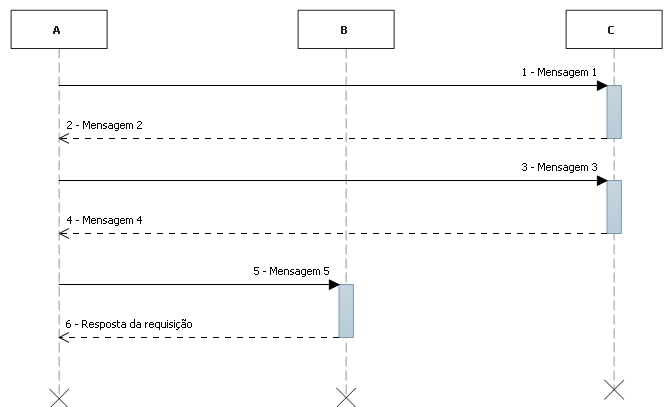
\includegraphics[width=0.8\textwidth]{fluxo_autenticacao_BAN.png}
    \caption{Diagrama de idealização do protocolo de autenticação/autorização proposto}
    \label{fig:protocoidealizado}
\end{figure}

\begin{enumerate}
  \item Mensagem 1: $\Msg{A}{C}{\Encrypt{Ts_A,Cred_A,H{\Encrypt{Msg_{AC}}{Ka ^{-1}}}}{Kc}}$.
  \item Mensagem 2: $\Msg{C}{A}{\Encrypt{Ts_C,{N_{CA}},H{\Encrypt{Msg_{CA}}{Kc ^{-1}}}}{Ka}}$.
  \item Mensagem 3: $\Msg{A}{C}{\Encrypt{Ts_A,{Resp_{AC}},Cod_{Srv_A},H{\Encrypt{Msg_{AC}}{Ka ^{-1}}}}{Kc}}$.
  \item Mensagem 4: $\Msg{C}{A}{\Encrypt{Ts_C,Exp_A,\#(\ShareSecret{A}{{C_{Aut}}}{C}),H{\Encrypt{Msg_{CA}}{Kc ^{-1}}}}{Ka}}$.
  \item Mensagem 5: $\Msg{A}{B}{\Encrypt{Ts_A,(\ShareSecret{A}{{C_{Aut}}}{C}),H{\Encrypt{Msg_{AB}}{Ka ^{-1}}}}{Ka}},{Req_A}$.
\end{enumerate}
\subsection{Suposições}\label{sec:Suposicoes}
O objetivo do protocolo é fazer que a entidade ${A}$ seja autenticada pela entidade ${C}$ e obtenha uma credencial de autenticação e autorização temporária referente a uma requisição de um serviço que a entidade ${A}$ deseja consumir. De forma que a credencial de autenticação e autorização temporária  possa ser utilizada pela entidade ${A}$ no momento da requisição do serviço a entidade ${B}$ e obtenha o que deseja. Para isso, algumas suposições iniciais são estabelecidas e juntamente com a aplicação  dos postulados da lógica BAN, busca-se concluir que o protocolo alcance o objetivo proposto. Todas as suposições, apresentadas na Tabela~\ref{tab:suposicoesBAN} são baseadas em um canal seguro de comunicação SSL/TSL, onde tanto o receptor  quanto o emissor do serviço são conhecidos e autenticados usando-se certificados digitais X.509.

\begin{table}[h]
\begin{tabular}{cllcl}
\textbf{Suposição} & \textbf{Descrição} &  & \textbf{Suposição} & \textbf{Descrição} \\
\textbf{1 -}       & $ A \mid\equiv$  ${\PubKey{Kc}{C}}$                 &  & \textbf{9 -}       & $ B \mid\equiv$ $ C \Rightarrow $ $\#(\ShareSecret{A}{{C_{Aut}}}{C})$ \\
\textbf{2 -}       & $ B \mid\equiv$  ${\PubKey{Ka}{A}}$                 &  & \textbf{10 -}      & $ A \mid\equiv$ $ C \mid\equiv $ $\#(\ShareSecret{A}{{C_{Aut}}}{C})$ \\
\textbf{3 -}       & $ C \mid\equiv$  ${\PubKey{Ka}{A}}$                 &  & \textbf{11 -}      & $ B \mid\equiv$ $ C \mid\equiv $ $\#(\ShareSecret{A}{{C_{Aut}}}{C})$ \\

\textbf{4 -}       & $ A \mid\equiv$  $\#{Ts_C}$                         &  & \textbf{12 -}      & $ A \mid\equiv$  $\#(\ShareSecret{A}{{C_{Aut}}}{C})$  \\

\textbf{5 -}       & $ B \mid\equiv$  $\#{Ts_A}$                         &  & \textbf{13 - }      & $ B \mid\equiv$  $\#(\ShareSecret{A}{{C_{Aut}}}{C})$  \\

\textbf{6 -}       & $ C \mid\equiv$  $\#{Ts_A}$                         &  & \textbf{ }                    &                                      \\
\textbf{7 -}       & $ A \mid\equiv$  ${Exp_A}$                          &  & \textbf{ }                   &
\\
\textbf{8 -}       & $ A \mid\equiv$  $ C \Rightarrow $ $\#(\ShareSecret{A}{{C_{Aut}}}{C})$   &   & \textbf{ }     &                               \\
\end{tabular}
\caption {Suposições aplicadas ao protocolo proposto.}
\label{tab:suposicoesBAN}
\end{table}


Dessa forma, temos que as suposições 1,2 e 3 garantem que as entidades participantes ${A}$, ${B}$ e ${C}$ confiam  nas chaves públicas das entidades que farão as trocas de mensagem. As suposições 4, 5 e 6 são \emph{timestamps}, o que denota que as entidades ${A}$, ${B}$ e ${C}$ devem estar sincronizadas. Sendo assim, a entidade ${A}$ acredita que o \emph{timestamp} ${Ts_C}$ é novo e foi gerado recentemente. Da mesma forma que as entidades ${B}$ e ${C}$ acreditam  que o \emph{timestamp} ${Ts_A}$ também é novo e foi gerado recentemente. A suposição 7 é utilizada pela entidade ${A}$ para garantir que a credencial de autenticação e autorização gerado pela entidade ${C}$ não expirou e que pode ser utilizada. As suposições 8 e 9 denotam que as entidades ${A}$, ${B}$ acreditam que entidade ${C}$ tem jurisdição  sobre a credencial de autenticação e autorização gerada. Portanto, as suposições 10 e 11 garantem que as entidades ${A}$, ${B}$ acreditam que a credencial de autenticação e autorização gerada é nova é foi realmente gerada pela entidade ${C}$. Finalmente, as suposições 12 e 13 garantem que as entidades ${A}$, ${B}$ acreditam na nova credencial de autenticação e autorização temporária, ${C_{Aut}}$.

\subsection{Provas}

Como o objetivo final do protocolo é autenticar a entidade ${A}$, de forma que ela obtenha uma credencial de autenticação e autorização temporária, referente a uma requisição de serviço desejado. Será realizado uma análise de cada mensagem  do protocolo idealizado. Para isso, serão aplicados os postulados lógicos e suposições, a fim de provar que o protocolo consegue atingir o objetivo proposto.

Na primeira mensagem, a entidade ${A}$ envia sua credencial, um \emph{timestamp} e o código do serviço que ele está querendo consumir ao servidor de autenticação e autorização, representado pela entidade ${C}$. A mensagem enviada é assinada com a chave privada do participante ${A}$  e cifrada com a chave pública do participante ${C}$. Esse processo e descrito a seguir:

\textbf{Mensagem 1}: $\Msg{A}{C}{\Encrypt{Ts_A,Cred_A,H{\Encrypt{Msg_{AC}}{Ka ^{-1}}}}{Kc}}$.

$C\triangleleft$ ${\Encrypt{Ts_A,Cred_A,Cod_{Srv_A},H{\Encrypt{Msg_{AC}}{Ka ^{-1}}}}{Kc}}$

$C\mid\equiv A \mid\sim $  $H\{Msg_{AC}\}$

$C\mid\equiv A \mid\sim$ ${\#Ts_A}$

$C\mid\equiv$ ${Cred_A,Cod_{Srv_A}}$

Sendo assim, ${\textbf{C}}$ recebe a fórmula ${\Encrypt{Ts_A,Cred_A,Cod_{Srv_A},H{\Encrypt{Msg_{AC}}{Ka ^{-1}}}}{Kc}}$, e usando sua chave privada, decifra a fórmula recebida. Após decifrar a fórmula, e aplicando a regra do significado da mensagem na suposição 3 usando a função $H \{Msg_{AC}\}$ confirma a autenticidade e integridade da mensagem. Por fim, aplica a regra de verificação do identificador na suposição 6 usando a fórmula ${Ts_A}$ para obter a credencial da entidade ${A}$ :  ${Cred_A}$.

Resultado:

${C}$ obtém  a credencial da entidade $A$: ${Cred_A}$

Na segunda mensagem, após receber e validar os dados enviados por $A$, a entidade ${C}$ gera um desafio de autenticação, ${N_{CA}}$. O desafio consiste em fazer uma busca aleatória à tabela de credenciais e selecionar um código de credencial que esteja associado a entidade $A$. Em seguida grava-se o desafio, a data e hora de geração do desafio e a resposta esperada em uma base de dados. Na sequência, uma mensagem, contendo o desafio e um \emph{timestamp}, é enviada a entidade $A$, assinada com a chave privada da entidade ${C}$ e cifrada com a chave pública da entidade ${A}$. Logo temos:

\textbf{Mensagem 2}: $\Msg{C}{A}{\Encrypt{Ts_C,{N_{CA}},H{\Encrypt{Msg_{CA}}{Kc ^{-1}}}}{Ka}}$.

$\textbf{A}\triangleleft$ ${\Encrypt{Ts_C,{N_{CA}},H{\Encrypt{Msg_{CA}}{Kc ^{-1}}}}{Ka}}$

$\textbf{A}\mid\equiv \textbf{C} \mid\sim $  $H \{Msg_{CA}\}$

$\textbf{A}\mid\equiv \textbf{C} \mid\sim$ ${Ts_C}$

$\textbf{A}\mid\equiv$ ${N_{CA}}$

A entidade ${\textbf{A}}$ recebe a fórmula ${\Encrypt{Ts_C,{N_{CA}},H{\Encrypt{Msg_{CA}}{Kc ^{-1}}}}{Ka}}$ e a decifra usando sua chave privada, em seguida aplicando a regra do significado da mensagem na suposição 1 usando a função $H \{Msg_{CA}\}$ confirma a autenticidade e integridade da mensagem. Por fim, aplica a regra de verificação do identificador na suposição 4 e usando a fórmula ${Ts_C}$ para obter o desafio,${N_{CA}}$, gerado pela entidade ${C}$.

Resultado:

${A}$ obtém  o desafio de autenticação gerado pela entidade ${C}$: ${N_{CA}}$

Na terceira mensagem, a entidade ${A}$, após receber e validar o desafio gerado pela entidade ${C}$, envia a resposta ${Resp_{AC}}$, conforme solicitado. Essa resposta consiste em informar o código do desafio gerado pela entidade ${C}$ e a credencial associada ao código de credencial solicitada pela entidade ${C}$. Além disso, a entidade ${A}$ deve informar o código do serviço que deseja consumir. Sendo assim, temos:

\textbf{Mensagem 3}: $\Msg{A}{C}{\Encrypt{Ts_A,{Resp_{AC}},Cod_{Srv_A},H{\Encrypt{Msg_{AC}}{Ka ^{-1}}}}{Kc}}$.

$C\triangleleft$ ${\Encrypt{Ts_A,{Resp_{AC}},H{\Encrypt{Msg_{AC}}{Ka ^{-1}}}}{Kc}}$

$C\mid\equiv A \mid\sim $  $H \{Msg_{AC}\}$

$C\mid\equiv A \mid\sim$ ${\#Ts_A}$

$C\mid\equiv$ ${Resp_{AC}}$

${\textbf{C}}$ recebe a fórmula ${\Encrypt{Ts_A,{Resp_{AC}},H{\Encrypt{Msg_{AC}}{Ka ^{-1}}}}{Kc}}$, e a decifra usando sua chave privada, em seguida aplicando a regra do significado da mensagem na suposição 3 usando a função $H \{Msg_{AC}\}$ confirma a autenticidade e integridade da mensagem. Por fim, aplica a regra de verificação do identificador na suposição 6 usando a fórmula ${Ts_A}$ para obter os dados da resposta do desafio ${Resp_{AC}}$, e assim, validar a resposta enviada e autenticar a entidade ${A}$. Dando início ao processo de autorização.

Resultado:

${C}$ autentica a entidade ${A}$.

Na mensagem 4, após autenticar a entidade ${A}$, a entidade ${C}$ procede com o processo de autorização, que consiste em verificar qual serviço a entidade está querendo consumir, para isso verifica o código de serviço solicitado pela entidade ${A}$, $Cod_{Srv_A}$, que foi informado no envio da mensagem 3. Se a entidade ${A}$ possuir privilégios necessários para consumir o serviço requisitado, a entidade ${C}$ gera uma nova credencial de autorização temporária para o serviço solicitado. Em seguida, a entidade ${C}$ grava a credencial ${(\ShareSecret{A}{{C_{Aut}}}{C})}$, o código do serviço que a entidade ${A}$ está requerendo, a data e hora de criação, a data de expiração e o código do contrato da entidade ${A}$. Terminado esse procedimento, a entidade ${C}$, envia, uma mensagem contendo a credencial ${(\ShareSecret{A}{{C_{Aut}}}{C})}$, a data e hora de expiração da credencial,${Exp_A}$ e um \emph{timestamp} a entidade ${A}$. Esta mensagem é assinada com a privada da entidade ${C}$ e cifrada com a chave pública da entidade ${A}$. Logo temos:

\textbf{Mensagem 4}: $\Msg{C}{A}{\Encrypt{Ts_C,Exp_A,\#(\ShareSecret{A}{{C_{Aut}}}{C}),H{\Encrypt{Msg_{CA}}{Kc ^{-1}}}}{Ka}}$.

$\textbf{A}\triangleleft$ $\Msg{C}{A}{\Encrypt{Ts_C,Exp_A,\#(\ShareSecret{A}{{C_{Aut}}}{C}),H{\Encrypt{Msg_{CA}}{Kc ^{-1}}}}{Ka}}$.

$\textbf{A}\mid\equiv \textbf{C} \mid\sim $  $H \{Msg_{CA}\}$

$\textbf{A}\mid\equiv \textbf{C} \mid\sim$ ${Ts_C}$

$\textbf{A}\mid\equiv \textbf{C} \mid\sim$ ${Exp_A}$

$\textbf{A}\mid\equiv \textbf{C} \Rightarrow $  ${\#(\ShareSecret{A}{{C_{Aut}}}{C})}$

$\textbf{A}\mid\equiv \textbf{C} \mid\equiv $  ${\#(\ShareSecret{A}{{C_{Aut}}}{C})}$

$\textbf{A}\mid\equiv$ ${\#(\ShareSecret{A}{{C_{Aut}}}{C})}$

A entidade ${A}$ recebe a fórmula ${\Encrypt{Ts_C,Exp_A,\#(\ShareSecret{A}{{C_{Aut}}}{C}),H{\Encrypt{Msg_{CA}}{Kc ^{-1}}}}{Ka}}$, e a decifra usando sua chave privada, em seguida aplicando a regra do significado da mensagem na suposição 1 usando a função $H \{Msg_{CA}\}$ confirma a autenticidade e integridade da mensagem. Ela aplica a regra de verificação do identificador nas suposições 4 e 7 usando as fórmulas ${Ts_C}$  e ${Exp_A}$. E, finalmente, aplicando a regra da jurisdição, nas suposições 7 e 9, obtém a credencial de autorização temporária ${\#(\ShareSecret{A}{{C_{Aut}}}{C})}$.

Resultado:

${\textbf{A}}$ obtém a credencial de autorização temporária: ${\#(\ShareSecret{A}{{C_{Aut}}}{C})}$.

Finalmente, na quinta mensagem, a entidade ${A}$ após receber e validar a mensagem enviada pela entidade ${C}$, obtendo assim a credencial de autenticação e autorização temporária, ${\#(\ShareSecret{A}{{C_{Aut}}}{C})}$, envia uma mensagem a entidade ${B}$  contendo a requisição do serviço que deseja consumir juntamente com a credencial de autorização temporária. Esta mensagem é assinada com a chave privada da entidade ${A}$ e cifrada com a chave pública da entidade ${B}$. Logo temos:

\textbf{Mensagem 5}: $\Msg{A}{B}{\Encrypt{Ts_A,(\ShareSecret{A}{{C_{Aut}}}{C}),H{\Encrypt{Msg_{AB}}{Ka ^{-1}}}}{Kb}},{Req_A}$.

$\textbf{B}\triangleleft$  ${\Encrypt{Ts_A,(\ShareSecret{A}{{C_{Aut}}}{C}),H{\Encrypt{Msg_{AB}}{Ka ^{-1}}}}{Kb}},{Req_A}$

$\textbf{B}\mid\equiv \textbf{A} \mid\sim $  $H\{Msg_{AB}\}$

$\textbf{B}\mid\equiv \textbf{A} \mid\sim$ ${Ts_A}$

$\textbf{B}\mid\equiv \textbf{A} \Rightarrow $  ${\#(\ShareSecret{A}{{C_{Aut}}}{C})}$

$\textbf{B}\mid\equiv \textbf{A} \mid\equiv $  ${\#(\ShareSecret{A}{{C_{Aut}}}{C})}$

$\textbf{B}\mid\equiv$ ${\#(\ShareSecret{A}{{C_{Aut}}}{C})}$

A entidade ${\textbf{B}}$ recebe a fórmula ${\Encrypt{Ts_A,(\ShareSecret{A}{{C_{Aut}}}{C}),H{\Encrypt{Msg_{AB}}{Ka ^{-1}}}}{Kb}},{Req_A}$, e a decifra, usando sua chave privada. Em seguida aplicando a regra do significado da mensagem na suposição 2 usando a função $H\{Msg_{AB}\}$ confirma a autenticidade e integridade da mensagem. Ela aplica a regra de verificação do identificador na suposições 5 usando as fórmulas ${Ts_A}$. E, finalmente, aplicando a regra da jurisdição, nas suposições 8 e 10, obtém a credencial de autorização temporária ${\#(\ShareSecret{A}{{C_{Aut}}}{C})}$ e autoriza a entidade \textbf{A} a consumir a requisição ${Req_A}$.

Conclusão :

${B}$ autoriza ${A}$ a partir da nova credencial ${(\ShareSecret{A}{{C_{Aut}}}{C})}$ a consumir a requisição ${Req_A}$

\subsection{Análise}

A análise demonstra que o protocolo de autenticação e autorização proposto alcança os objetivos propostos na Seção~\ref{sec:Suposicoes}, que é a autenticação da entidade ${A}$ e a emissão da credencial de autenticação e autorização temporária. Isso permite que a entidade ${A}$ consuma o serviço requerido. É importante frisar que a lógica BAN foi utilizada para demonstrar a execução do protocolo e que a utilização da lógica é apenas um dos passos necessários para verificar se existem possíveis falhas no protocolo.

Para verificar a segurança do protocolo é necessário que seja empregado um método de criptoanálise sobre a criptografia utilizada e assim verificar quais são vulnerabilidades que o protocolo ou os algoritmos criptográficos empregados estão sujeitos.


\section{Implementação}\label{sec:implementacao}

Após a definição do protocolo proposto e para atender a necessidade da realização de testes de desempenho que tem a finalidade de avalizar o impacto da solução proposta no oferecimento de serviços pela PCDF, surgiu a necessidade da criação de um protótipo do protocolo de autenticação e autorização proposto. Esse protótipo foi desenvolvido em conjunto com o corpo acadêmico da UNB, neste caso, o responsável pelo desenvolvimento foi o aluno Alexandre Lucchesi.  A descrição desse protótipo e apresentado a seguir.
\subsection{Protótipo}

Para implementar o protótipo do protocolo proposto foi necessário desenvolver cada um dos componentes: Cliente, Servidor de Autenticação e Autorização e Servidor REST, descritos na arquitetura do protocolo na seção~\ref{sec:ArqProtocolo}. Para isso, foi utilizada a linguagem de programação puramente funcional Haskell, com o compilador GHC(Glasgow Haskell Compiler) versão 7.6.3. Para o controle de dependências e gerenciamento de \emph{build} de aplicações foi utilizado à ferramenta Cabal que é um o gerenciador de pacotes do Haskell. Com ele é possível construir aplicações e bibliotecas de forma padronizada, organizada e portável. Para criar o protótipo ainda foi utilizado o framework Haskell para desenvolvimento web, denominado Snap \emph{Framework} que é necessário para manipulação de requisições e respostas HTTP, que são utilizadas pelo protocolo de autenticação e autorização proposto. Além disso, foi utilizado o HsOpenSSL que é um OpenSSL vinculativo para Haskell, utilizado para garantir a utilização do HTTPS em todas as trocas de mensagem a partir de código Haskell.

Para a assinatura digital das mensagens utilizadas pelo protocolo foi utilizado o algoritmo RSASSA\-PKCS\-v1\_5 SHA\-256 conforme orientação descrita na publicação~\cite{ietfjws} e para criptografia foi utilizado o algoritmo de criptografia assimétrica, RSAES\-PKCS1\-V1\_5, para cifrar a chave simétrica utilizada no algoritmo de criptografia simétrica AES\_128\_CBC\_HMAC\_SHA\_256 que foi utilizado para cifrar a mensagem. Procurou-se seguir a orientação do que é preconizado na publicação~\cite{jwt2014}.

O servidor de banco de dados foi implementado utilizando o banco de dados não relacional \emph{Apache CouchDB}, que é um banco de dados flexível e tolerante a falhas que usa \emph{JSON} para armazenar os dados, JavaScript como sua linguagem de consulta usando o MapReduce, além disso, este banco de dados oferece API estilo REST.

O protótipo implementado não objetivou a otimização do protocolo, seu objetivo foi o de possibilitar a realização dos testes de desempenho e de verificar as funcionalidades do protocolo proposto.

\section{Análise de Segurança}

Nesta seção serão discutidas as propriedades de segurança do protocolo de autenticação e autorização proposto. São abordadas as propriedades e alguns ataques que podem ser realizados contra ele. Essa seção segue o padrão determinado no trabalho~\cite{traust08}.

\subsection{Segurança da sessão}

O protocolo de Autenticação e Autorização proposto utiliza para segurança de seção e da camada de transporte, o protocolo TLS/SSL. A utilização desse protocolo tem por objetivo evitar o ataque man-in-the-middle. Para isso, é exigido tanto do órgão conveniado como da própria PCDF que ambas utilizem certificados digitais padrão X.509 emitidos e garantidos por uma AC que esteja subordinada à hierarquia da ICP-Brasil.

Com isso, ambas as partes envolvidas no processo de comunicação podem estabelecer um processo de confiança mútua no nível de transporte. Todo o tráfego que flui sobre uma sessão bilateral certificada tem uma fonte confiável. Isso permite que implementações de serviços possam autorizar ou desautorizar interações com base na fonte bem conhecida de uma solicitação HTTP.

Além da segurança oferecida pela utilização da segurança na camada de transporte, com utilização do TLS/SSL, o protocolo utiliza mecanismos de segurança tais como criptografia assimétrica e assinatura digital. Isso Permite que outras partes mal intencionadas não consigam ter acesso ao conteúdo das mensagens trocadas pelo protocolo no processo de comunicação.

Diferentemente do sistema Traust, o protocolo de Autenticação e Autorização proposto, não será executado em ambientes em que nem o cliente nem o servidor tem uma chave pública certificada, procura-se dessa forma, atenuar problemas relacionados ao protocolo TLS, que quando executado em ambientes em que nem o cliente nem o servidor tem uma chave pública certificada, pode ser vulnerável a um ataque man-in-the-middle durante o estabelecimento da sessão~\cite{traust08}.

\subsection{Responsabilização dos usuários conveniados}

Uma das ameaças verificadas diz respeito a possibilidade do uso indevido, por parte dos órgãos conveniados, das informações disponibilizadas nos serviços ofertados pela PCDF. Isso decorre do fato das informações disponibilizadas serem sensíveis e possuírem caráter sigiloso. Dessa forma, para evitar esse problema é exigido dos órgãos conveniados que assinem um contrato para o consumo do serviço. No momento da assinatura do contrato eles recebem uma tabela contendo várias credenciais que servem como identidades e que deverão ser utilizadas no processo de autenticação, conforme descrito no seção~\ref{sec:reqprotocolo}. Isso possibilita que haja uma autenticação mútua entre a PCDF e os consumidores dos serviços. Além disso, com a utilização do protocolo de autenticação e autorização proposto, são empregados mecanismos de criptografia e assinaturas digitais que são geradas a partir de certificados digitais padrão X.509 vinculados aos órgãos e garantidos por AC. Dessa forma, busca-se evitar o não-repúdio por parte dos órgãos conveniados, atribuindo-lhes responsabilidades em caso do mau uso dos serviço ofertados pela PCDF.

Logo, uma vez detectado algum tipo de vazamento de dados proveniente dos serviços ofertados o órgão poderá ser identificado e após uma apuração minuciosa, responsabilizado pelos danos causados à PCDF.

\subsection{Ataques de repetição}
Esta ameaça, conforme descrito no capitulo~\ref{cap:revisaolit}, seção~\ref{sec:vulnerabilidadessoa}, se empregada contra o protocolo de autenticação e autorização proposto, tem uma chance quase nula de sucesso. Uma vez que são empregados \emph{timestamps} em em todas as trocas de mensagens realizadas pelo protocolo. Além disso, são gerados números únicos, que identificam os desafios de autenticação gerados e podem ser utilizados como \emph{nonces}, que também podem ser empregados contra esse tipo de ataque.

\subsection{Ataques de negação de serviço}

Esta ameaça é muito difícil de ser evitada, haja vista que,  pode ser fruto de ataques via rede, do consumo excessivo de recursos da máquina,  ou ainda,  ser resultante da exploração de qualquer tipo de vulnerabilidade que implique na indisponibilidade do serviço ou de um recurso. O protocolo de autenticação e autorização proposto é baseado no esquema de desafio-resposta. Os desafios são gerados de forma aleatória a partir das credenciais que identificam unicamente os consumidores dos serviços, o que possibilita uma autenticação mútua. Além disso, também são empregados outros mecanismos de segurança como utilização da segurança na camada de transporte e mecanismos de criptografia e assinaturas digitais. Isso minimiza a ameaça de ataques de negação de serviço.

Assim como o sistema Traust,~\cite{traust08}, o servidor de autenticação e autorização proposto pode ser replicado para outros servidores, o que possibilita um balanceamento de carga e minimiza a criação de gargalos. Isso permite que o servidor de autenticação seja escalável e esteja disponível em situações críticas, como no caso dos ataques de negação de serviço.


\subsection{Roubo de credenciais de autenticação e autorização}\label{subsec:RouboCred}

O protocolo de autenticação a autorização proposto após executado corretamente emite um token de segurança que será utilizado para a obtenção do serviço desejado, conforme apresenato na seção~\ref{sec:ArqProtocolo}, cabe ressaltar que se por algum motivo um atacante, conseguir burlar o os mecanismos de segurança utilizados pelo protocolo e conseguir acesso a essa credencial de autenticação e autorização ele terá acesso apenas um serviço, pois o protocolo emite credenciais para um único serviço por vez e com tempo de expiração determinado no momento de sua geração.

Essa é uma situação muito difícil de ser verificada, porém caso ocorra o problema é minimizado e não terá grande impacto na arquitetura do protocolo como um todo.

Outro problema que pode ocorrer é o roubo de credenciais de autenticação, que são as credenciais que o órgão conveniado recebe no momento da assinatura do contrato de oferecimento do serviço. Essa credenciais são utilizadas para responder os desafios que serão realizadas pelo protocolo de autenticação proposto. Caso isso ocorra e seja identificado a PCDF pode de forma rápida e transparente desativar as credenciais que julgar que foram comprometidas sem que o usuário seja prejudicado. Em um caso mais extremo, outras podem ser geradas e redistribuíras ao órgão conveniado.

Porém cabe ressaltar que caso ocorra o roubo de credenciais, o órgão que teve o problema será investigado e poderá ser responsabilizado se for detectado má fé má gestão na guarda das credenciais, conforme descrito na subseção~\ref{subsec:RouboCred}


\subsection{Ponto único de ataque}

Uma das possibilidades verificadas é que ocorrendo um ataque, o alvo possa não ser protocolo de autenticação e autorização proposto e sim o próprio servidor de autenticação e autorização. Neste caso, se o atacante for bem sucedido em sua empreitada o servidor poder ficar vulnerável. Esse servidor é responsável pela geração dos desafios de autenticação e pela geração das credenciais de autenticação e autorização. Porém, apesar de realizar estas atividades ele armazena e consulta os dados gerados no processo de autenticação e autorização em outra máquina, que é em um servidor de banco de dados. Em outras palavras o servidor de autenticação e autorização está em uma máquina diferente do servidor de banco de dados, o que minimiza os problemas relacionados a esse tipo de ataque, pois o servidor pode ser replicado para outra máquina e o que estiver com problemas pode ser fácilmente substituído.
\section{Síntese do capítulo}

Este capítulo apresentou os requisitos e a arquitetura do protocolo de autenticação e autorização proposto.  Além disso,  o capítulo apresentou a formalização do protocolo utilizando à lógica BAN.  Foi descrita de forma sucinta a implementação de um protótipo do protocolo proposto. Ao final foi realizada uma análise de segurança semelhante ao do trabalho proposto em~\cite{traust08}. No próximo capítulo será realizada uma análise de desempenho a fim de mensurar o impacto do protocolo na infraestrutura da PCDF. 